\chapter{METHODOLOGY}
\label{ch:methodology}

\hs This chapter presents the methodology adopted for the design, development, and evaluation of the proposed Python libraries, namely \GradientCOBRA{} and \KFCProcedure{}. The objective of this study is to transform consensus-based aggregation and clusterwise supervised learning methods from theoretical formulations into reusable and modular machine learning frameworks.

The study follows a design and development research methodology. It begins with a review of related aggregation and clusterwise learning methods, followed by requirements analysis, system architecture design, framework construction, and experimental validation. This approach focuses on the conceptual workflow of the proposed frameworks, the interaction between their major components, and the evaluation protocol used to assess their predictive performance.

The functional scope of the proposed system is divided into two main pipelines. The first pipeline is the \GradientCOBRA{} subsystem, which implements prediction-space aggregation through consensus-based learning. It includes regression aggregation through \GradientCOBRA{}, mixed input-output aggregation through \textbf{MixCOBRARegressor}, and classification aggregation through \textbf{CombinedClassifier}. The second pipeline is the \KFCProcedure{} framework, which implements clusterwise supervised learning by integrating divergence-based clustering, local predictive modeling, and final prediction aggregation.

Although the two frameworks can operate independently, they can also be combined in a hybrid configuration. In this configuration, the prediction matrix generated by the \KFCProcedure{} clusterwise pipeline can be used as input to COBRA-based combiners. This allows clusterwise local learning and prediction-space aggregation to be studied within a unified methodological workflow.

Detailed implementation aspects, including source-code structure, class organization, package layout, and engineering decisions, are discussed separately in Chapter~\ref{ch:implementation}.



% ============================== RESEARCH METHODOLOGY
\section{Research Methodology}
\label{sec:research_methodology}

\hs This study adopts a design and development research methodology to implement, validate, and evaluate two advanced machine learning frameworks: \GradientCOBRA{} and \KFCProcedure{}. The primary objective is to convert theoretical aggregation and clusterwise learning methods into reusable and extensible Python libraries that follow modern machine learning workflows.

The research process consists of five sequential phases, as illustrated in \figref{fig:research_workflow}.

\begin{enumerate}
    \item \textbf{Literature Review and Requirements Analysis:} A review of ensemble learning, consensus-based aggregation, kernel-based aggregation, and clusterwise learning was conducted to identify the methodological requirements of the proposed frameworks. This phase established the need for modular distance functions, kernel weighting, optimization routines, divergence-based clustering, local model training, and final aggregation mechanisms.

    \item \textbf{System Architecture Design:} Based on the identified requirements, two complementary architectures were designed. The COBRA subsystem was structured around prediction-space similarity and kernel-weighted aggregation, while the \KFCProcedure{} subsystem was structured around input-space decomposition, cluster-local modeling, and prediction fusion.

    \item \textbf{Framework Construction:} The frameworks were developed around reusable methodological components, including splitters, estimators, normalizers, distances, kernels, losses, optimizers, aggregators, Bregman divergences, local models, and combiners. The focus of this chapter is on the methodological role of these components rather than their detailed source-code implementation.

          % \item \textbf{Experimental Validation:} The frameworks were validated using experiment notebooks for regression and classification tasks. These notebooks verify that the proposed systems can be trained, combined with baseline models, and evaluated under repeated random splits.

          % \item \textbf{Performance Evaluation:} Predictive performance was assessed using task-appropriate metrics. Classification notebooks use accuracy, precision, recall, and F1-score, while regression notebooks use metrics such as MAE, MSE, RMSE, MAPE, and $R^2$, depending on the dataset notebook.

    \item \textbf{Experimental Validation:} The frameworks were validated through experimental workflows for regression and classification tasks. These experiments verify that the proposed systems can be trained, combined with baseline models, and evaluated under repeated random splits.

    \item \textbf{Performance Evaluation:} Predictive performance was assessed using task-appropriate metrics. Classification experiments use accuracy, precision, recall, and F1-score, while the reported regression results use MAPE, RMSE, $R^2$, and the average test-target value, depending on the dataset. MAE and MSE are implemented as loss functions but are not included in the final regression result tables.

\end{enumerate}

The overall methodology therefore bridges theoretical machine learning methods and practical validation. It emphasizes how the proposed components interact within complete training and prediction workflows, while detailed implementation and software organization are discussed separately in Chapter~\ref{ch:implementation}.

\begin{figure}[H]
    \centering
    \resizebox{\textwidth}{!}{%
        \begin{tikzpicture}[
                node distance=2.2cm,
                every node/.style={
                        draw,
                        align=center,
                        minimum width=4.2cm,
                        minimum height=2.2cm
                    }
            ]
            \node (r1) {Literature Review\\and Requirements Analysis};
            \node (r2) [right=of r1] {Software\\Architecture Design};
            \node (r3) [right=of r2] { Framework\\Construction};
            \node (r4) [right=of r3] {Experimental\\Validation};
            \node (r5) [right=of r4] {Performance\\Evaluation};

            \draw[->] (r1) -- (r2);
            \draw[->] (r2) -- (r3);
            \draw[->] (r3) -- (r4);
            \draw[->] (r4) -- (r5);
        \end{tikzpicture}%
    }
    \caption{Research Methodology Workflow}
    \label{fig:research_workflow}
\end{figure}

% ============================== SYSTEM ARCHITECTURE

\section{System Architecture}
\label{sec:system_architecture}

\hs The proposed system consists of two related machine learning frameworks: \KFCProcedure{} and the COBRA aggregation subsystem centered on \GradientCOBRA{}. Each framework is designed as an independent predictive system, but they can also be combined through the aggregation stage of the \KFCProcedure{} pipeline.

\subsection{Independent Framework Design}

\hs \KFCProcedure{} is a clusterwise supervised learning framework designed to model heterogeneous data distributions through explicit input-space partitioning. Its learning process follows three main stages: clustering, local model training, and prediction aggregation. First, the input space is partitioned under one or more Bregman divergences. Then, separate local models are trained within each divergence-specific cluster. Finally, the divergence-level predictions are combined into a single global output.

\GradientCOBRA{} is a prediction-space aggregation framework. Instead of partitioning the original feature space, it constructs a prediction matrix from multiple base estimators or receives such a prediction matrix directly. It then computes distances between prediction vectors, transforms these distances into kernel weights, optimizes aggregation parameters, and produces final predictions through weighted aggregation.

From a methodological perspective, \KFCProcedure{} emphasizes \textit{input-space decomposition and local specialization}, while \GradientCOBRA{} emphasizes \textit{prediction-space similarity and kernel-based aggregation}. These two approaches are complementary: one creates localized predictive views of the data, and the other combines multiple predictive views through a data-dependent weighting mechanism.

\subsection{Hybrid System Configuration}

\hs Beyond their independent operation, the two frameworks can be integrated into a hybrid architecture, as illustrated in \figref{fig:hybrid}.

\begin{figure}[H]
    \centering
    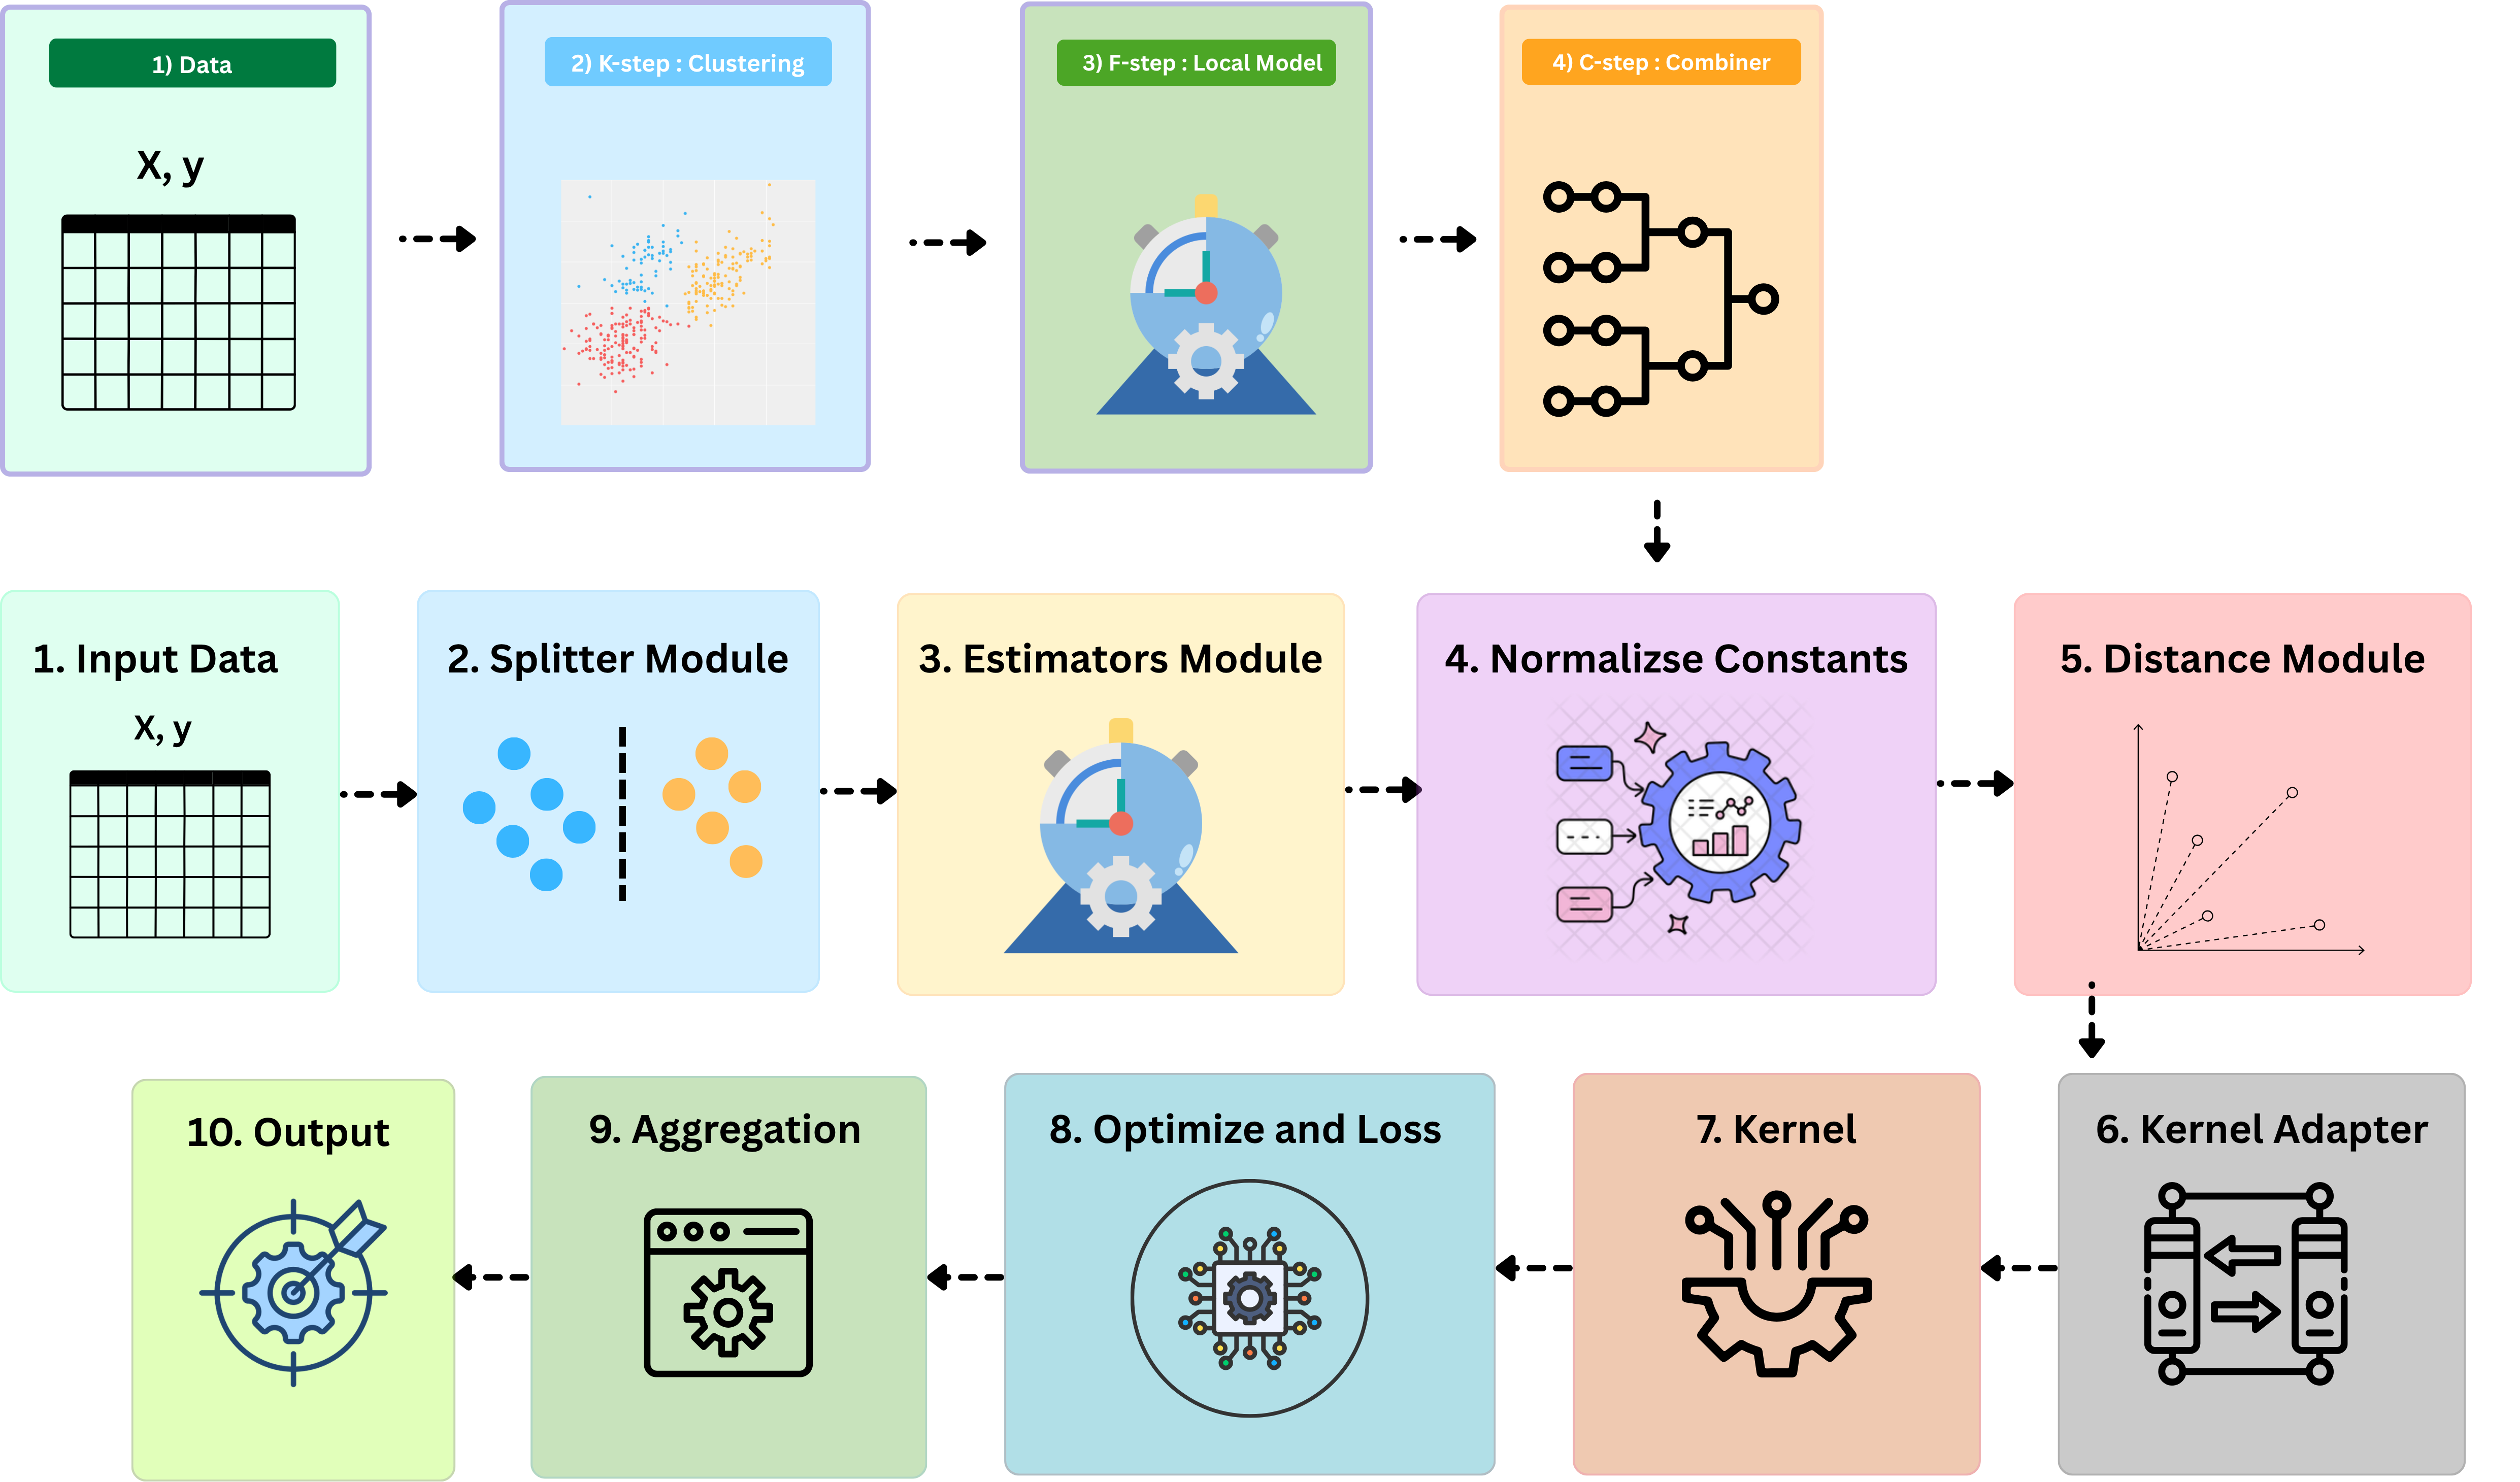
\includegraphics[width=0.75\textwidth]{figures/architectures/hybrid.png}
    \caption{Hybrid System Architecture}
    \label{fig:hybrid}
\end{figure}

In this configuration, \KFCProcedure{} acts as the lower-level prediction generation framework. For each divergence, samples are assigned to clusters, routed to the corresponding local models, and transformed into a divergence-level prediction vector. These prediction vectors are stacked into a prediction matrix. The C-step can then use a COBRA-based combiner, such as \textbf{CombinedClassifier}, \GradientCOBRA{}, or \textbf{MixCOBRARegressor}, to aggregate this matrix.

% Consequently, the hybrid system should not be viewed as a rigid sequence in which \KFCProcedure{} is required to call \GradientCOBRA{} directly. Instead, COBRA-based aggregation is supported by the repository as one potential C-step approach within the \KFCProcedure{} architecture. This design allows clusterwise local learning and prediction-space aggregation to interact within a single methodological workflow.


Consequently, the hybrid system should not be viewed as a rigid sequence in which \KFCProcedure{} is required to call \GradientCOBRA{} directly. Instead, COBRA-based aggregation is supported as one possible C-step strategy within the \KFCProcedure{} architecture. This design allows clusterwise local learning and prediction-space aggregation to interact within a unified methodological workflow.



% ============================ GradientCobra

\section{Design of the GradientCOBRA Ensemble Framework}
\label{sec:gradientcobra_design}


\hs The \GradientCOBRA{} subsystem is designed as a modular framework for consensus-based aggregation in prediction space. The developed library provides three main predictive variants: \GradientCOBRA{} for regression aggregation in prediction space, \textbf{MixCOBRARegressor} for regression aggregation using both input-space and prediction-space distances, and \textbf{CombinedClassifier} for classification aggregation through weighted voting.


The architecture follows a layered design in which individual methodological responsibilities are separated into independent components. Core functionalities such as data splitting, estimator management, distance computation, kernel transformation, optimization, loss evaluation, and aggregation are defined as interchangeable modules. This design enables the framework to support different aggregation strategies without changing the overall learning workflow. \figref{fig:gradientcobra_architecture} illustrates the conceptual architecture of the \GradientCOBRA{} subsystem.

\begin{figure}[H]
    \centering
    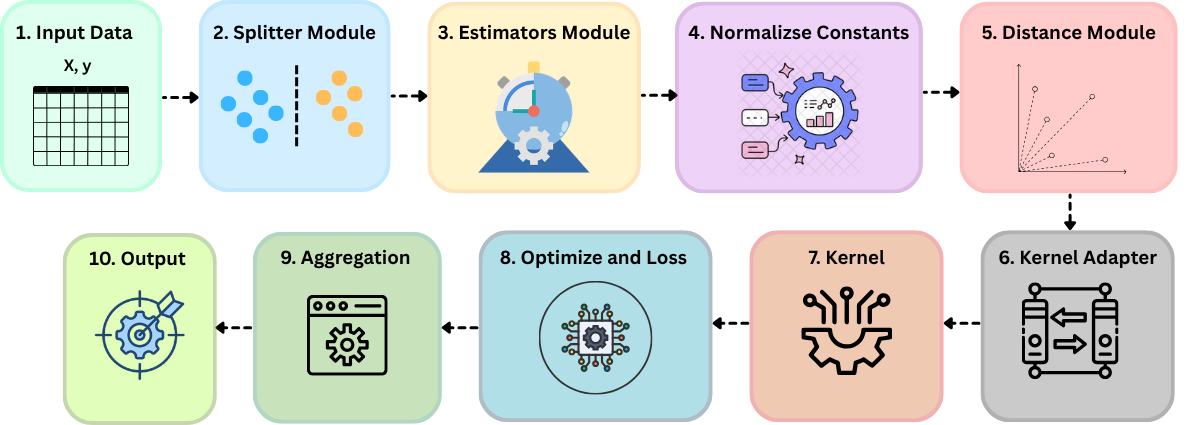
\includegraphics[width=0.85\textwidth]{figures/architectures/gradientcobra.png}
    \caption{GradientCOBRA Ensemble Framework}
    \label{fig:gradientcobra_architecture}
\end{figure}

The framework consists of ten modules:

\begin{enumerate}
    \item \textbf{Splitters Module:} Manages the construction of training and calibration partitions.
    \item \textbf{Estimators Module:} Responsible for training, configuring, or resolving predictive models that produce the prediction matrix.
    \item \textbf{Normalizers Module:} Derives normalization constants to standardize prediction outputs and improve comparability across estimators.
    \item \textbf{Distance Module:} Provides a collection of distance measures for quantifying dissimilarity between observations, including Euclidean, Manhattan, Cosine, Hamming, and Minkowski distances.
    \item \textbf{Adapters Module:} Applies parameterized transformations to distance matrices before kernel evaluation, supporting both automatically learned parameters and externally supplied parameter values.
    \item \textbf{Kernel Module:} Maps adapted distance values to similarity weights through kernel-based function transformations.
    \item \textbf{Optimizer Module:} Selects aggregation parameters, such as bandwidths and mixing coefficients, using search-based or gradient-based optimization techniques.
    \item \textbf{CV Module:} Provides cross-validation frameworks for evaluating and selecting aggregation parameters based on predictive performance.
    \item \textbf{Loss Module:} Defines objective functions that quantify model performance and guide parameter selection procedures.
    \item \textbf{Aggregators Module:} Produces the final prediction using weighted mean for regression or weighted vote for classification.
\end{enumerate}

These subsystems are coordinated by the main COBRA variants. Each variant follows a unified principle: it constructs or receives a prediction space, computes similarities between query and calibration samples, and aggregates calibration targets based on kernel-derived weights.

\subsection{Splitters Module}
\label{subsec:splitters_module}

\hs The Splitters module provides the data partitioning mechanism used in COBRA-style aggregation. It separates the data used to train base estimators from the data used for calibration. This separation is essential because the aggregation layer is evaluated using predictions computed on a reference set that is later used for kernel-based weighting.

\subsubsection*{Functional Role in the Framework}

Two splitting strategies are supported. The first is a random holdout mechanism that generates disjoint training and calibration sets. The second is an overlap-based strategy, in which a configurable proportion of samples is shared between the two subsets. This design enables flexible trade-offs between estimator diversity and calibration data availability.

An \textbf{as\_predictions} mode is also provided, allowing the framework to operate directly on a precomputed prediction matrix. In this mode, estimator training is omitted, enabling seamless integration with external prediction generators such as \KFCProcedure{}.

\subsubsection*{Mathematical Formulation}

Let $D = \{(x_i, y_i)\}_{i=1}^{n}$. The splitter defines two index sets $I_K$ and $I_L$ corresponding to estimator training and calibration, respectively. In the holdout case, $I_K \cap I_L = \emptyset$, whereas in the overlap case $I_K \cap I_L \neq \emptyset$, with the degree of overlap governed by a user-defined parameter. The calibration subset $(X_L, y_L)$ is used as the reference set for kernel-weighted aggregation.

\subsection{Estimators Module}
\label{subsec:estimators_module}

\hs The Estimators module constitutes the primary machine learning component of the COBRA framework. It is responsible for training individual base learners (referred to as ``machines'') and organizing their prediction outputs. Consistent with prior work on ensemble consensus efficiency \cite{ali2015, cagnini2023}, the module is designed to accommodate heterogeneous predictive models, enabling the combination of diverse learning algorithms, including linear models, tree-based ensembles, and neighborhood methods, within a unified aggregation framework.


\subsubsection*{Mathematical Formulation}
From a mathematical perspective, the Estimators module can be viewed as a vector-valued mapping function. Let there be $M$ base estimators configured within the module: $\{m_1, m_2, \dots, m_M\}$. Given an input vector $x \in \mathbb{R}^d$, each individual estimator provides a localized prediction: $f_j(x) = m_j(x), \ \forall j \in \{1, 2, \dots, M\}$. When an entire matrix of validation or testing data $X \in \mathbb{R}^{n \times d}$ is provided, the module applies each estimator to every sample, producing a prediction matrix, $\hat{Y}$:
\[
    \hat{Y} = \begin{bmatrix}
        f_1(x_1) & f_2(x_1) & \dots  & f_M(x_1) \\
        f_1(x_2) & f_2(x_2) & \dots  & f_M(x_2) \\
        \vdots   & \vdots   & \ddots & \vdots   \\
        f_1(x_n) & f_2(x_n) & \dots  & f_M(x_n)
    \end{bmatrix} \in \mathbb{R}^{n \times M}
\]
This matrix $\hat{Y}$ represents the transformed data structure that is subsequently passed into the weight-optimization or kernel-mapping stages of the framework.

\subsection{Normalizer Module}
\label{subsec:normalizer_module}

\hs The Normalizer module applies scalar normalization to prediction outputs generated by base estimators, ensuring stable computation of distances in prediction space.

In addition, the developed library provides standalone feature normalization methods, including standard scaling and min-max normalization. These utilities are implemented as reusable components; however, the primary training procedures of \GradientCOBRA{} and \textbf{MixCOBRARegressor} mainly rely on scalar normalization constants.


\subsubsection*{Mathematical Formulation}

For \GradientCOBRA{}, a scalar normalization constant is computed as:

\[
    c = \frac{s}{\max(|y|) \cdot M},
\]

where $s$ is a scale factor or user-provided normalization constant, $y$ is the target vector, and $M$ is the number of prediction columns. The prediction matrix $P$ is then transformed as:

\[
    \tilde{P} = cP.
\]

For \textbf{MixCOBRARegressor}, two scalar normalizations are used: one for the input space and one for the prediction space. This allows the input-distance component and prediction-distance component to be combined within a comparable numerical range.

Standalone feature-level normalizers are also available:

\paragraph{Standard Normalizer}
\[
    \tilde{Y}_{i,j} = \frac{Y_{i,j} - \mu_j}{\sigma_j + \epsilon}
\]

\paragraph{Min-Max Normalizer}
\[
    \tilde{Y}_{i,j} = \frac{Y_{i,j} - \min_j}{\max_j - \min_j + \epsilon}
\]

These normalizers support reusable preprocessing but should not be confused with the scalar normalization constants used directly inside the main COBRA training pipelines.

\subsection{Kernel Adapter Module}
\label{subsec:kernel_adapter_module}

\hs The Kernel Adapter module transforms distance matrices before they are passed to the kernel function. Its role is not to normalize final aggregation weights, but to control the scale and combination of distances. This distinction is important because weight normalization or fallback behavior is handled later by the aggregator.

\subsubsection*{Mathematical Formulation}

For a one-parameter adapter, used by \GradientCOBRA{} and one-parameter configurations of \textbf{MixCOBRARegressor}, the adapted distance is defined as:


\[
    D^{\prime} = hD,
\]

where $D$ is the raw distance matrix and $h$ is the bandwidth parameter selected through optimization.

For a two-parameter adapter, used in the two-space form of \textbf{MixCOBRARegressor}, the adapted distance combines input-space and prediction-space distances:

\[
    D^{\prime} = \alpha D_X + \beta D_Y,
\]

where $D_X$ is the input-space distance matrix, $D_Y$ is the prediction-space distance matrix, and $\alpha$ and $\beta$ are mixing parameters selected during optimization. The adapted distance $D^{\prime}$ is then transformed by a kernel function to produce similarity weights.

\subsection{Kernel Module}
\label{subsec:kernel_module}

\hs While the Kernel Adapter module handles scaling, bandwidth control, and structural transformation of distance values, the Kernel module implements the core kernel functions that map adapted distances into similarity weights. It isolates kernel evaluation into a dedicated component, ensuring both computational clarity and modularity in the aggregation process.

The Kernel module operates on pre-adapted non-negative distances $D \ge 0$ and produces similarity weights via a kernel function $K(\cdot)$. A summary of the supported kernel functions is provided in \tabref{tab:kernel_functions}. A visual comparison of selected kernel shapes is presented in \figref{fig:kernel_function_shapes}, showing how each kernel maps distance values to aggregation weights.


\subsubsection*{Mathematical Formulation}

Let $D \ge 0$ denote a pre-adapted distance value. The Kernel module computes similarity weights as:
\[
    W = K(D),
\]
where $K(\cdot)$ is selected from a predefined set of kernel functions implemented via the \textbf{KernelFactory} interface (see \tabref{tab:kernel_functions}).

\begin{table}[H]
    \centering
    \renewcommand{\arraystretch}{1.4}
    \setlength{\extrarowheight}{2pt}
    \begin{tabularx}{\textwidth}{|l|c|X|}
        \hline
        \textbf{Kernel}                             & \textbf{Expression} & \textbf{Description}       \\
        \hline

        COBRA (Threshold)                           &
        $K(D) = \mathbf{1}_{\{D < h\}}$             &
        Hard selection kernel used in classical COBRA; activates only within bandwidth $h$.            \\
        \hline


        Radial Basis Function (RBF) &
        $K(D) = \exp(-D^2)$ &
        Gaussian-style smooth decay kernel used in \GradientCOBRA{}; default continuous weighting kernel. \\
        \hline


        Epanechnikov                                &
        $K(D) = \max(1 - D, 0)$                     &
        Compact-support linear kernel with finite influence radius.                                    \\
        \hline

        Reverse Cosh                                &
        $K(D) = \cosh(D)^{-\nu}$                    &
        Smooth kernel with tunable decay controlled by $\nu > 0$.                                      \\
        \hline

        Cauchy                                      &
        $K(D) = \frac{1}{1 + D^2}$                  &
        Heavy-tailed kernel robust to large distances.                                                 \\
        \hline

        Biweight                                    &
        $K(D) = (1 - D^2)^2 \mathbf{1}_{\{D < 1\}}$ &
        Smooth compact-support kernel with quadratic decay.                                            \\
        \hline

        Triweight                                   &
        $K(D) = (1 - D^2)^3 \mathbf{1}_{\{D < 1\}}$ &
        Higher-order smooth compact-support kernel.                                                    \\
        \hline

        Triangular                                  &
        $K(D) = \max(1 - |D|, 0)$                   &
        Simple linear decay kernel with finite support.                                                \\
        \hline

        Exponential                                 &
        $K(D) = \exp(-D)$                           &
        Standard exponential decay kernel.                                                             \\
        \hline
    \end{tabularx}
    \caption{Kernel functions supported in the Kernel module.}
    \label{tab:kernel_functions}
\end{table}

\begin{figure}[H]
    \centering
    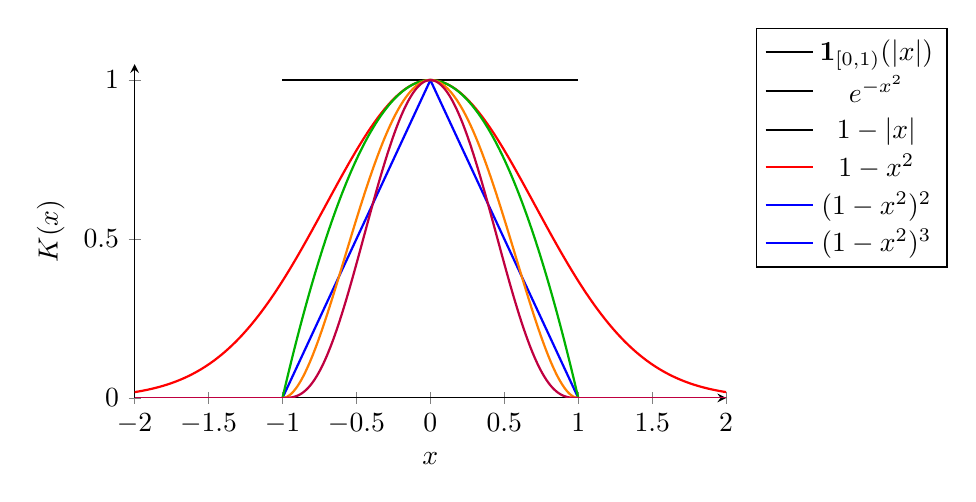
\begin{tikzpicture}
        \begin{axis}[
                width=0.75\textwidth,
                height=0.48\textwidth,
                xmin=-2, xmax=2,
                ymin=0, ymax=1.05,
                xlabel={$x$},
                ylabel={$K(x)$},
                axis lines=left,
                grid=none,
                legend style={
                        at={(1.05,0.75)},
                        anchor=west,
                        draw=black,
                        fill=white
                    },
                samples=300,
                domain=-2:2
            ]

            % COBRA threshold / uniform kernel
            \addplot[black, thick, domain=-1:1] {1};
            \addplot[black, thick, domain=-2:-1] {0};
            \addplot[black, thick, domain=1:2] {0};
            \addlegendentry{$\mathbf{1}_{[0,1)}(|x|)$}

            % Gaussian / RBF
            \addplot[red, thick] {exp(-x^2)};
            \addlegendentry{$e^{-x^2}$}

            % Triangular
            \addplot[blue, thick, domain=-1:1] {1 - abs(x)};
            \addplot[blue, thick, domain=-2:-1] {0};
            \addplot[blue, thick, domain=1:2] {0};
            \addlegendentry{$1-|x|$}

            % Epanechnikov
            \addplot[green!70!black, thick, domain=-1:1] {1 - x^2};
            \addplot[green!70!black, thick, domain=-2:-1] {0};
            \addplot[green!70!black, thick, domain=1:2] {0};
            \addlegendentry{$1-x^2$}

            % Biweight
            \addplot[orange, thick, domain=-1:1] {(1 - x^2)^2};
            \addplot[orange, thick, domain=-2:-1] {0};
            \addplot[orange, thick, domain=1:2] {0};
            \addlegendentry{$(1-x^2)^2$}

            % Triweight
            \addplot[purple, thick, domain=-1:1] {(1 - x^2)^3};
            \addplot[purple, thick, domain=-2:-1] {0};
            \addplot[purple, thick, domain=1:2] {0};
            \addlegendentry{$(1-x^2)^3$}

        \end{axis}
    \end{tikzpicture}
    \caption{Shapes of kernel functions used for distance-to-weight transformation}
    \label{fig:kernel_function_shapes}
\end{figure}

As illustrated in \figref{fig:kernel_function_shapes}, the threshold kernel performs hard selection by assigning equal weight within a fixed interval and zero weight outside it. In contrast, smooth kernels such as the Gaussian, Epanechnikov, biweight, triweight, and triangular kernels gradually reduce the influence of observations as the distance increases.


\subsection{Optimizer Module}
\label{subsec:optimizer_module}

\hs The Optimizer module selects the numerical parameters governing kernel-based aggregation. Depending on the COBRA variant, these parameters include a bandwidth $h$ for \GradientCOBRA{} and \textbf{CombinedClassifier}, or a pair of mixing coefficients $(\alpha, \beta)$ for \textbf{MixCOBRARegressor} that balance input-space and prediction-space distances.

The optimization strategy is model-dependent. The \textbf{CombinedClassifier} uses grid search exclusively. In contrast, \GradientCOBRA{} and \textbf{MixCOBRARegressor} support both grid search and gradient-based optimization, where applicable. When gradient-based optimization is not supported by the selected kernel or objective function, the framework defaults to grid search.

\subsubsection*{Mathematical Formulation}

Let $\theta$ denote the aggregation parameter vector. For \GradientCOBRA{}, $\theta$ may be the bandwidth $h$. For \textbf{MixCOBRARegressor}, $\theta$ may be $(\alpha,\beta)$. The optimizer selects:

\[
    \theta^* = \arg\min_{\theta} \frac{1}{K}\sum_{k=1}^{K}
    \mathcal{L}\left(y_{\mathrm{val}}^{(k)}, \hat{y}_{\theta}^{(k)}\right),
\]

where $\mathcal{L}$ is the selected loss function and the predictions $\hat{y}_{\theta}^{(k)}$ are obtained by kernel-weighted aggregation over the calibration folds.

\subsection{Cross-Validation (CV) Module}
\label{subsec:validators_module}

\hs The CV module supplies cross-validation strategies used during bandwidth optimization within \GradientCOBRA{}. Rather than a monolithic validator, the module provides three factory-registered splitters: \textbf{KFoldCV} for standard i.i.d.\ data, \textbf{StratifiedKFoldCV} for class-balanced classification settings, and \textbf{TimeSeriesCV} for chronological temporal data. Each splitter exposes a unified iterator interface that yields \textbf{SplitIndices} objects containing training and evaluation index sets, ensuring zero data leakage across folds.

\subsection{Loss Module}
\label{subsec:loss_module}

\hs The Loss module defines the formal optimization objectives. It accommodates differentiable and continuous functions required for gradient evaluations, alongside standard evaluation criteria.

\subsubsection*{Mathematical Formulation}
The module implements six concrete loss functions. For regression tasks, Mean Squared Error (MSE) and Mean Absolute Error (MAE) provide standard objectives, while Huber loss and Quantile loss provide robust alternatives. For classification tasks, Log Loss and Hinge Loss are implemented. The core regression losses are defined as:
\[
    L_{\mathrm{MSE}}(y, \hat{y}) = \frac{1}{n}\sum_{i=1}^n (y_i - \hat{y}_i)^2, \quad
    L_{\mathrm{MAE}}(y, \hat{y}) = \frac{1}{n}\sum_{i=1}^n |y_i - \hat{y}_i|
\]
The Huber loss combines quadratic and linear behavior, controlled by a transition parameter $\delta > 0$:
\[
    L_{\mathrm{Huber}}(y_i, \hat{y}_i) =
    \begin{cases}
        \tfrac{1}{2}(y_i - \hat{y}_i)^2                          & \text{if } |y_i - \hat{y}_i| \le \delta \\
        \delta\bigl(|y_i - \hat{y}_i| - \tfrac{1}{2}\delta\bigr) & \text{otherwise}
    \end{cases}
\]

\subsection{Aggregators Module}
\label{subsec:aggregators_module}

\hs The Aggregators module serves as the final step in the execution pipeline. It implements two factory-registered strategies: \textbf{WeightedMeanAggregator} for regression tasks and \textbf{WeightedVoteAggregator} for classification tasks. Both operate on kernel-derived weight vectors and validation target values.

\paragraph{Weighted Mean (Regression)}
Given a weight vector $W \in \mathbb{R}^n$ and target values $y \in \mathbb{R}^n$, the aggregated prediction is:
\[
    \hat{f}(x) = \frac{\sum_{i=1}^n W_i y_i}{\sum_{i=1}^n W_i}
\]
If the weight sum is zero, the aggregator falls back to the arithmetic mean of $y$.

\paragraph{Weighted Vote (Classification)}
For discrete class labels $\mathcal{C}$, the aggregator assigns each class a weighted support score and returns the class with maximum accumulated weight:
\[
    \hat{f}(x) = \arg\max_{c \in \mathcal{C}} \sum_{i=1}^n W_i \cdot \mathbf{1}_{\{y_i = c\}}
\]

\subsection{COBRA Predictive Variants}
\label{subsec:cobra_predictive_variants}

\hs The developed library provides three main COBRA-style predictive variants: \GradientCOBRA{}, \textbf{MixCOBRARegressor}, and \textbf{CombinedClassifier}.

\paragraph{\GradientCOBRA{}}

\GradientCOBRA{} is a regression method that operates in the prediction space. It either trains a set of base estimators and constructs their prediction matrix, or receives a precomputed prediction matrix through prediction-space mode. Distances are computed between prediction vectors, transformed into kernel weights, and used to aggregate calibration targets through a weighted mean.

\paragraph{\textbf{MixCOBRARegressor}}

\textbf{MixCOBRARegressor} extends prediction-space aggregation by incorporating both input-space and prediction-space distances. Its methodological motivation is that samples may be considered similar not only when base estimators produce similar predictions, but also when they are close in the original feature space. The two-space formulation is expressed as:

\[
    D^{\prime}(x_i, x_j) = \alpha D_X(x_i, x_j) + \beta D_Y(p_i, p_j),
\]

where $D_X$ is the input-space distance, $D_Y$ is the prediction-space distance, and $\alpha$ and $\beta$ control their relative contributions.

\paragraph{\textbf{CombinedClassifier}}

\textbf{CombinedClassifier} adapts the COBRA aggregation principle to classification tasks. Instead of aggregating continuous target values through a weighted mean, it aggregates class labels through weighted voting. The default prediction-space distance for classification is Hamming distance, which is suitable for comparing vectors of classifier outputs. The final class is selected as the class with the largest accumulated kernel-weighted support.

\subsection{Algorithmic Pipeline}

\begin{algorithm}[H]
    \caption{COBRA-Style Training and Prediction Pipeline}
    \label{alg:gradientcobra}
    \begin{algorithmic}[1]

        \Require Dataset $(X,y)$ or precomputed prediction matrix $P$
        \Require Distance function $d$, kernel $K$, adapter parameter $\theta$, aggregator $A$, loss $\mathcal{L}$
        \Ensure Trained aggregation model with optimized parameter $\theta^*$

        \State \textbf{1. Resolve training context}
        \If{raw features are provided}
        \State Split data into estimator-training subset $(X_K,y_K)$ and calibration subset $(X_L,y_L)$
        \State Fit base estimators on $(X_K,y_K)$
        \State Construct prediction matrix $P_L$ from base-estimator outputs on $X_L$
        \Else
        \State Treat the input matrix as an existing prediction matrix $P_L$
        \State Use the associated target vector $y_L$ for calibration
        \EndIf

        \State \textbf{2. Normalize aggregation space}
        \State Compute scalar normalization constant $c$
        \State $\tilde{P}_L \leftarrow cP_L$

        \State \textbf{3. Compute calibration distances}
        \State $D_L \leftarrow d(\tilde{P}_L,\tilde{P}_L)$

        \State \textbf{4. Select aggregation parameter}
        \For{each candidate or optimizer step $\theta$}
        \State Adapt distances $D_{\theta}$
        \State Compute kernel matrix $W_{\theta} = K(D_{\theta})$
        \State Estimate cross-validation loss using weighted aggregation over calibration folds
        \EndFor
        \State Select $\theta^*$ with the lowest validation loss

        \State \textbf{5. Prediction}
        \State Construct or receive query prediction matrix $P^*$
        \State Normalize $P^*$ using the fitted scalar constant
        \State Compute distances between $P^*$ and $P_L$
        \State Apply the optimized adapter and kernel
        \State Aggregate $y_L$ using kernel weights

        \State \Return Final predictions

    \end{algorithmic}
\end{algorithm}



% =========================\KFCProcedure{}LIBRARY DESIGN

\section{Design of the \KFCProcedure{} Clusterwise Framework}
\label{sec:kfc_design}

\hs The \KFCProcedure{} framework is expected to be particularly suitable for datasets that satisfy two main assumptions. First, the input feature space should contain more than one latent cluster or subgroup, although the exact number of clusters is not assumed to be known in advance. Second, the predictive relationship within each cluster does not necessarily have to follow the same underlying model. In other words, different regions of the input space may be better represented by different local predictive functions. Under these conditions, a single global model may be insufficient, while a clusterwise learning strategy can decompose the problem into several local learning tasks and then combine their predictions through the C-step.


The overall architecture of the framework is illustrated in Figure~\ref{fig:kfc_architecture}, which presents the interaction between clustering, local modeling, and combiner components.

\begin{figure}[H]
    \centering
    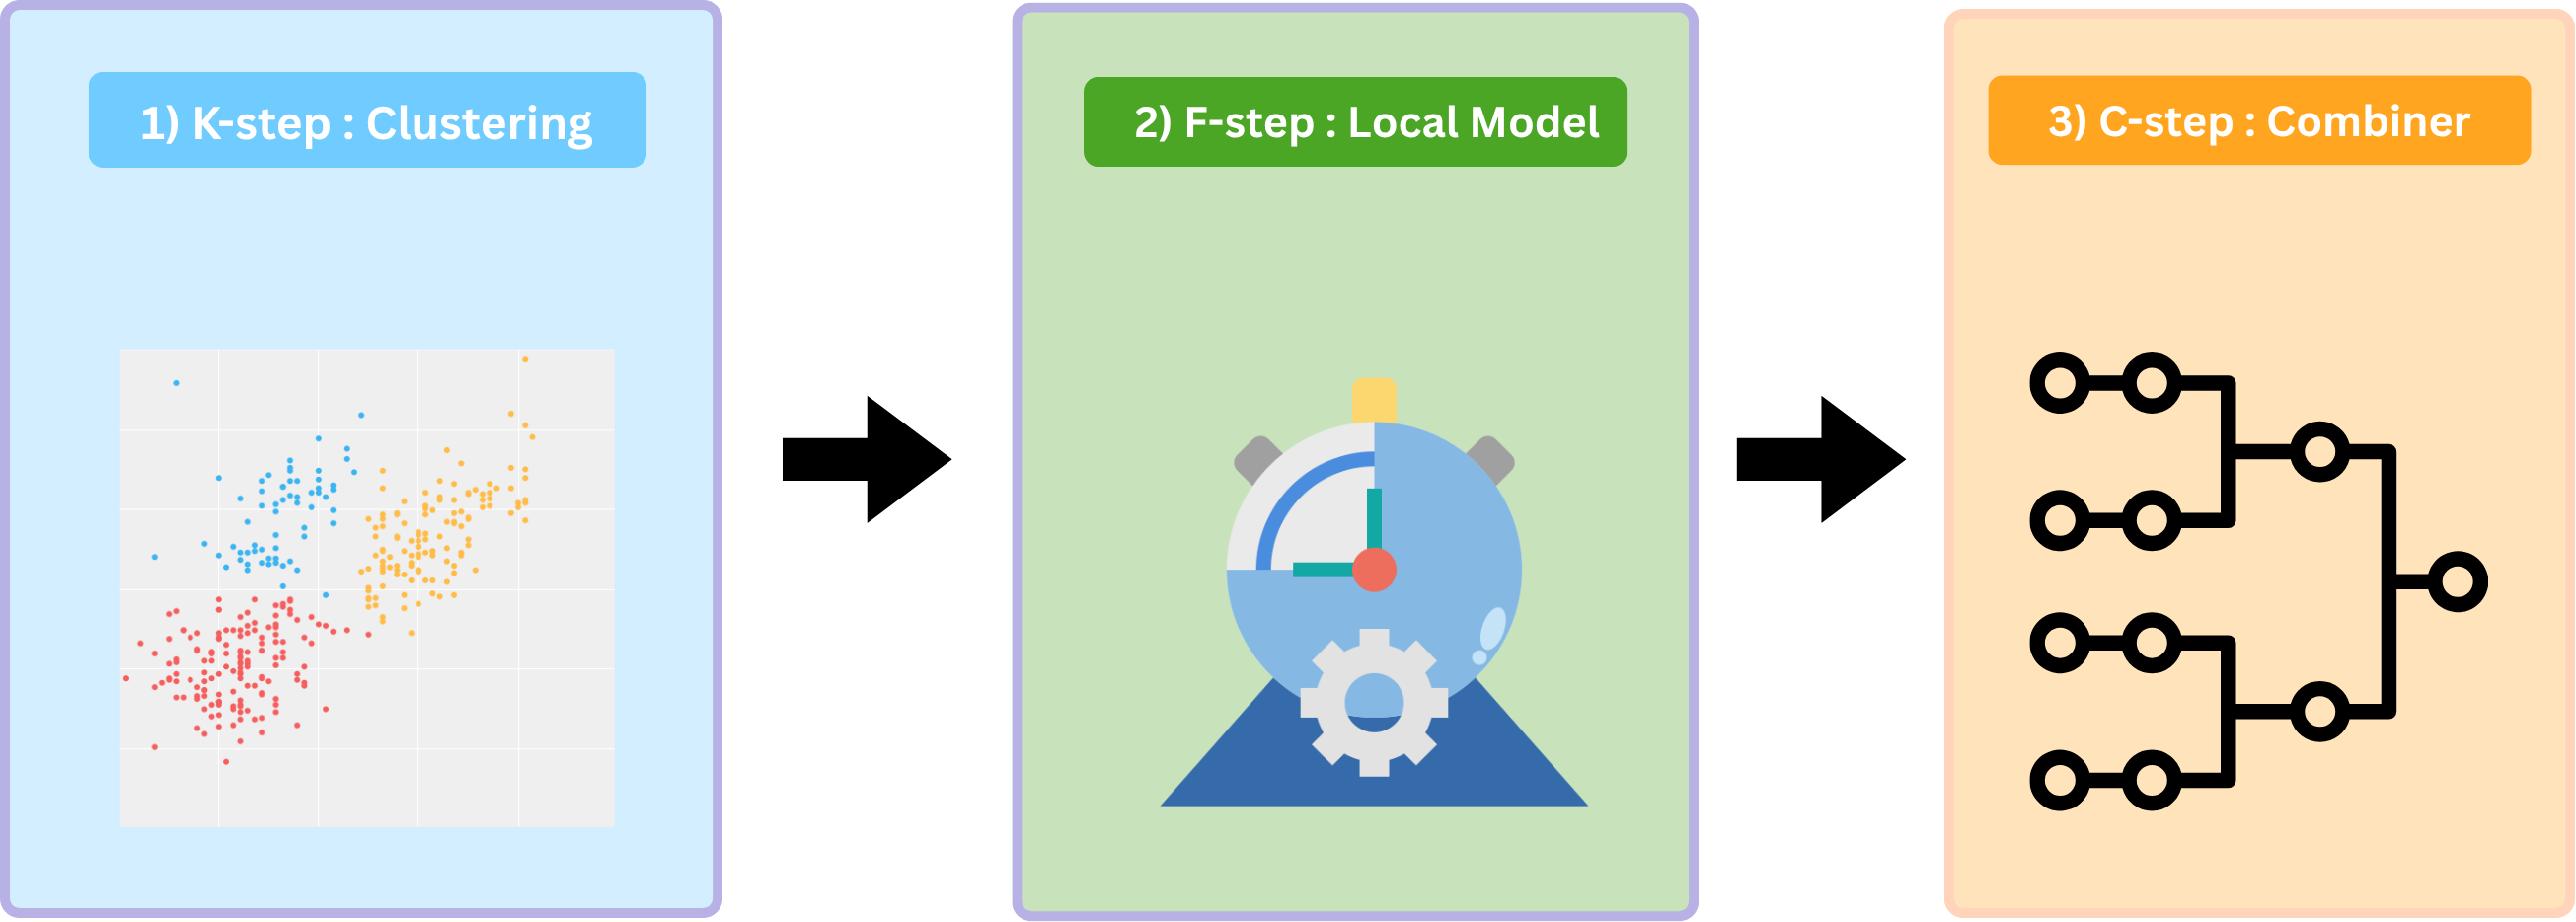
\includegraphics[width=0.85\textwidth]{figures/architectures/kfc.png}
    \caption{KFCProcedure Clusterwise Framework Architecture}
    \label{fig:kfc_architecture}
\end{figure}

The library is structured into three unified pipeline stages:

\begin{enumerate}
    \item \textbf{K-Step / Clustering Module:} For each divergence in a user-supplied divergence set $\mathcal{D}$, one Bregman K-Means model is fitted independently. This produces multiple divergence-specific partitions of the same input space.

    \item \textbf{F-Step / Local Model Module:} For each divergence and each cluster, a local estimator is trained using only the samples assigned to that cluster. This creates a collection of localized predictive models.

    \item \textbf{C-Step / Combiner Module:} During prediction, each divergence produces one prediction vector after samples are routed through their corresponding local cluster models. These vectors are stacked into a prediction matrix and aggregated into one final output.
\end{enumerate}


\subsection{Divergence-Based Clustering Module}

\hs The Clustering module represents the input-space decomposition stage of the \KFCProcedure{} framework. Its objective is to partition heterogeneous data into more coherent subregions before training local predictive models.

The module uses Bregman K-Means, which generalizes classical K-Means by replacing the standard Euclidean distance with a selected Bregman divergence. This allows the same dataset to be partitioned under different geometric assumptions. In the \KFCProcedure{} pipeline, each divergence produces a separate clustering hypothesis, which is later used to train divergence-specific local models.


\subsubsection*{Functional Role in the Framework}

Within the clusterwise learning pipeline, the Clustering module performs the following methodological roles:

\begin{itemize}
    \item \textbf{Feature-Space Partitioning:} The input matrix $X \in \mathbb{R}^{n \times d}$ is partitioned into $K$ clusters by minimizing divergence to learned centroids.

    \item \textbf{Multiple Geometric Views:} Each divergence produces its own partition of the same dataset, allowing the framework to represent the data under multiple similarity assumptions.

    \item \textbf{Routing Information:} The resulting cluster assignments are used by the F-step to decide which local model should be trained or applied for each sample.

    \item \textbf{Domain Validation:} Some divergences require specific input domains. The Euclidean divergence accepts real-valued inputs, while GKL and Itakura--Saito require positive values, and the logistic divergence requires values in the interval $(0,1)$.
\end{itemize}

\subsubsection*{Design Principles}

The clustering methodology follows three main principles:

\begin{itemize}
    \item \textbf{Divergence Modularity:} The clustering procedure is separated from the divergence function, allowing different Bregman divergences to be used without changing the overall K-step workflow.

    \item \textbf{Lloyd-Type Optimization:} The algorithm alternates between assigning samples to the closest centroid and updating centroids from assigned samples until convergence or a maximum iteration limit is reached.

    \item \textbf{Robust Cluster Formation:} Empty clusters are handled by reinitialization, which prevents the learning process from failing when a cluster receives no samples.
\end{itemize}

\subsubsection*{Mathematical Formulation}

Let $X = \{x_1, x_2, \dots, x_n\}$ be the input feature vectors, where $x_i \in \mathbb{R}^d$. A Bregman divergence generated by a strictly convex and differentiable function $\psi$ is defined as:

\[
    D_{\psi}(x_i, \mu_k) =
    \psi(x_i) - \psi(\mu_k)
    - \langle \nabla \psi(\mu_k), x_i - \mu_k \rangle.
\]

For each divergence $D_m \in \mathcal{D}$, the K-step assigns each sample to the closest centroid:

\[
    s_i^{(m)} = \arg\min_{k \in \{1, \dots, K\}} D_m(x_i, \mu_k^{(m)}).
\]

The developed library supports four divergence choices:

\begin{itemize}
    \item \textbf{Squared Euclidean} (\textbf{"euclidean"}), defined on real-valued data.
    \item \textbf{Generalized KL Divergence} (\textbf{"gkl"}), defined on positive-valued data.
    \item \textbf{Itakura--Saito Divergence} (\textbf{"is"}), defined on positive-valued data.
    \item \textbf{Logistic Loss Divergence} (\textbf{"logistic"}), defined on values strictly between 0 and 1.
\end{itemize}

\subsubsection*{Integration in the \KFCProcedure{} pipeline}

The Clustering module provides the structural partitions required by the Local Model module. During training, cluster assignments are computed for the K-step training subset. During prediction, new samples are assigned to their closest centroids under each divergence, and these assignments determine which local models are used in the F-step.

\subsection{Local Model Module}

\hs The Local Model module constitutes the F-step of the \KFCProcedure{} pipeline. Instead of fitting one global predictive model over the entire dataset, the framework trains local estimators inside the clusters produced by each divergence. This design supports piecewise modeling, where different regions of the input space may be represented by different predictive functions.

For each divergence $D_m$ and each cluster $k$, one local model is trained on the samples assigned to that cluster. During inference, each sample is routed to the local model associated with its predicted cluster under each divergence.

\subsubsection*{Functional Role in the Framework}

The Local Model module performs the following roles:

\begin{itemize}
    \item \textbf{Region-Specific Learning:} It trains independent estimators on cluster-conditioned subsets of the data.

    \item \textbf{Conditional Inference Routing:} During prediction, each sample is routed to one local model per divergence according to its cluster assignment.

    \item \textbf{Prediction Matrix Construction:} The F-step produces one prediction vector per divergence. These vectors are stacked into a matrix used by the C-step.
\end{itemize}

\subsubsection*{Mathematical Formulation}

Let $R_k^{(m)}$ denote the $k$-th cluster produced under divergence $D_m$. For each region, a local estimator $f_{m,k}$ is trained by minimizing a task-specific loss:

\[
    \theta_{m,k}^{*}
    =
    \arg\min_{\theta}
    \sum_{x_i \in R_k^{(m)}}
    \mathcal{L}\left(y_i, f_{m,k}(x_i;\theta)\right).
\]

For a query sample $x$, the prediction under divergence $D_m$ is:

\[
    \hat{y}^{(m)}(x)
    =
    f_{m,s^{(m)}(x)}(x),
\]

where $s^{(m)}(x)$ is the cluster assigned to $x$ under divergence $D_m$.

For $M$ divergences, the F-step output is the prediction matrix:

\[
    P =
    \begin{bmatrix}
        \hat{y}^{(1)}(x_1) & \hat{y}^{(2)}(x_1) & \cdots & \hat{y}^{(M)}(x_1) \\
        \hat{y}^{(1)}(x_2) & \hat{y}^{(2)}(x_2) & \cdots & \hat{y}^{(M)}(x_2) \\
        \vdots             & \vdots             & \ddots & \vdots             \\
        \hat{y}^{(1)}(x_n) & \hat{y}^{(2)}(x_n) & \cdots & \hat{y}^{(M)}(x_n)
    \end{bmatrix}.
\]

Thus, the C-step receives one column per divergence, not one column per cluster. The cluster models are used internally to produce each divergence-level prediction vector.

\subsubsection*{Integration in the Framework}

The Local Model module receives cluster labels from the K-step and produces the prediction matrix for the C-step. The current \KFCProcedure{} prediction workflow is based on class or value predictions from local models. Although some wrapped classifiers may support probability prediction individually, full probabilistic prediction through the \KFCProcedure{} pipeline is not fully established by the current F-step design and should not be presented as a completed methodological feature.

\subsection{Combiner Module}

\hs The Combiner module constitutes the C-step of the \KFCProcedure{} framework. After the F-step produces a prediction matrix, the combiner transforms multiple divergence-level predictions into one final output.

This module supports both regression and classification aggregation. Regression combiners include mean aggregation, weighted mean aggregation, stacking regression, \GradientCOBRA{}, and \textbf{MixCOBRARegressor}. Classification combiners include majority voting, stacking classification, and COBRA-based weighted voting through \textbf{CombinedClassifier}.


\subsubsection*{Functional Role in the Framework}

The Combiner module performs three main roles:

\begin{itemize}
    \item \textbf{Prediction Fusion:} It receives the F-step prediction matrix and produces one final prediction vector.

    \item \textbf{Task-Aware Aggregation:} It uses regression-specific strategies for continuous targets and classification-specific strategies for discrete labels.

    \item \textbf{Hybrid COBRA Integration:} It allows COBRA-based aggregation to be used directly inside the \KFCProcedure{} pipeline.
\end{itemize}

\subsubsection*{Mathematical Formulation}

Let $P(x)$ be the vector of divergence-level predictions for a sample $x$:

\[
    P(x) = \left[\hat{y}^{(1)}(x), \hat{y}^{(2)}(x), \dots, \hat{y}^{(M)}(x)\right].
\]

The combiner defines a mapping:

\[
    \hat{y}(x) = \mathcal{C}\left(P(x)\right),
\]

where $\mathcal{C}$ is the selected aggregation function.

\paragraph{Mean Aggregation}

\[
    \hat{y}(x) = \frac{1}{M}\sum_{m=1}^{M}\hat{y}^{(m)}(x).
\]

\paragraph{Weighted Linear Combination}

\[
    \hat{y}(x) = \sum_{m=1}^{M} w_m \hat{y}^{(m)}(x),
\]

where the weights are learned from the combiner training data.

\paragraph{Stacking Meta-Learning}

\[
    \hat{y}(x) = g(P(x)),
\]

where $g$ is a meta-model trained on the prediction matrix.

\paragraph{Majority Voting}

For classification, majority voting selects the most frequent predicted class among the divergence-level predictions:

\[
    \hat{y}(x) = \mathrm{mode}\left(\hat{y}^{(1)}(x), \dots, \hat{y}^{(M)}(x)\right).
\]

\paragraph{COBRA-Based Aggregation}

For COBRA-based combiners, the prediction matrix is treated as a prediction-space representation. Given calibration predictions $P_i$ and a query prediction vector $P(x)$, the combiner computes kernel weights:

\[
    w_i(x) = K\left(d(P(x), P_i)\right),
\]

and aggregates calibration targets using a weighted rule. For regression, this gives:

\[
    \hat{y}(x)
    =
    \frac{\sum_i w_i(x)y_i}{\sum_i w_i(x)}.
\]

For classification, the same idea is applied through weighted voting over class labels.

% \subsubsection{Integration in the Framework}

% The Combiner module is the final stage of KFCProcedure. It is fitted using the prediction matrix generated on the aggregation split and the corresponding targets. During inference, it receives the prediction matrix for new samples and returns the final global prediction.


\subsubsection*{Integration in the Framework}

The Combiner module represents the final stage of the \KFCProcedure{} pipeline. It is fitted using the prediction matrix generated from the aggregation split together with the corresponding target values. During inference, the module receives the prediction matrix produced for new samples and transforms it into the final predicted output.

\subsection{Algorithmic Pipeline}

\begin{algorithm}[H]
    \caption{KFCProcedure Training Procedure}
    \label{alg:kfc_training}
    \begin{algorithmic}[1]
        \Require Training dataset $(X,y)$
        \Require Divergence set $\mathcal{D}=\{D_1,\dots,D_M\}$
        \Require Number of clusters $K$
        \Require Local model family $f$
        \Require Combiner $C$

        \State Split $(X,y)$ into $(X_K,y_K)$ and $(X_L,y_L)$
        \State For classification tasks, preserve class balance during the split when possible

        \For{each divergence $D_m \in \mathcal{D}$}
        \State Fit Bregman K-Means on $X_K$ using divergence $D_m$
        \State Obtain training cluster assignments $S_K^{(m)}$
        \State Predict calibration cluster assignments $S_L^{(m)}$

        \For{each cluster $k=1,\dots,K$}
        \State Extract the local subset assigned to cluster $k$
        \State Train local model $f_{m,k}$ on this subset
        \EndFor

        \State Route samples in $X_L$ to their corresponding local models
        \State Generate one calibration prediction vector $p_L^{(m)}$
        \EndFor

        \State Form the calibration prediction matrix:
        \[
            P_L = \left[p_L^{(1)}, p_L^{(2)}, \dots, p_L^{(M)}\right]
        \]

        \State Fit combiner $C$ using $(P_L,y_L)$
        \State \Return Trained K-step, F-step, and C-step components
    \end{algorithmic}
\end{algorithm}

\hs During inference, a new input matrix $X^*$ is first assigned to clusters under each fitted divergence. The F-step then routes each sample to the corresponding local model and forms a new prediction matrix $P^*$. Finally, the fitted C-step combiner transforms $P^*$ into the final prediction vector.

% ========================= SOFTWARE ENGINEERING DESIGN PRINCIPLES

\section{Software Engineering Design Principles}
\label{sec:software_engineering_design}

\hs Although detailed implementation is discussed in Chapter~\ref{ch:implementation}, the methodological design of the two frameworks is guided by several software engineering principles. These principles are important because the objective of the study is not only to test an algorithm, but also to design reusable machine learning frameworks.

\subsection{Architectural Pattern Mapping}

\hs The frameworks are organized around interchangeable methodological components. Distances, kernels, losses, optimizers, divergences, local models, and combiners are treated as replaceable strategies. This design allows experiments to change one methodological component without changing the whole pipeline. Table~\ref{tab:pattern_mapping} summarizes how the main software engineering design principles are connected to the machine learning objectives of the proposed frameworks.

\begin{table}[H]
    \centering
    \caption{Mapping of Design Principles to Machine Learning Objectives}
    \label{tab:pattern_mapping}

    \begin{tabularx}{\textwidth}{l X X}
        \hline
        \textbf{Design Principle}                                          &
        \textbf{Framework Component}                                       &
        \textbf{Machine Learning Objective}                                                    \\
        \hline

        \textbf{Strategy-Based Design}                                     &
        Distances, kernels, divergences, losses, optimizers, and combiners &
        Enables alternative mathematical assumptions to be tested within the same workflow     \\

        \textbf{Modular Aggregation}                                       &
        COBRA aggregators and KFC combiners                                &
        Allows prediction fusion to be changed independently from base model training          \\

        \textbf{Separation of Stages}                                      &
        K-step, F-step, and C-step                                         &
        Separates clustering, local learning, and aggregation into clear methodological phases \\

        \textbf{Estimator-Style Interface}                                 &
        Main predictive classes                                            &
        Supports standard machine learning workflows based on fitting and prediction           \\
        \hline
    \end{tabularx}
\end{table}

\subsection{Scikit-Learn API Compliance}

\hs Both frameworks are designed around the common estimator workflow used in Python machine learning: models are initialized with configuration parameters, trained through a \textbf{fit} procedure, and used for inference through a \textbf{predict} procedure. Some classification components also provide probability outputs when supported by their internal estimators. However, probability prediction should be presented only for components where it is fully supported by the current framework, such as the COBRA classification aggregator, and not as a guaranteed feature of every \KFCProcedure{} configuration.

% =============================== EXPERIMENTAL DESIGN

\section{Experimental Design}
\label{sec:experimental_design}

\hs This section describes the experimental design used to evaluate the implemented \KFCProcedure{} framework. The purpose of the experiments is not only to compare predictive performance, but also to verify that the proposed framework can be trained, executed, and evaluated consistently across different supervised learning tasks. The experimental workflow includes dataset preparation, preprocessing, model configuration, repeated train--test evaluation, and performance reporting.

The experiments are divided into two main task groups: classification and regression. For classification, the proposed models are compared with standard baseline classifiers and a standalone aggregation classifier. For regression, the proposed models are compared with standard baseline regressors and COBRA-based aggregation regressors. This design allows the framework to be assessed under different data types, target variables, and prediction objectives.

\subsection{Experimental Environment}

\hs The experimental implementation was conducted using Python in a notebook-based environment. The datasets were retrieved using \textbf{kagglehub}, while data processing and numerical computation were performed using \textbf{pandas} and \textbf{numpy}. Exploratory analysis and visualization were supported by \textbf{matplotlib} and \textbf{seaborn}. Standard preprocessing tools, baseline models, data splitting functions, and evaluation metrics were provided by \textbf{scikit-learn}.

The main framework components imported from the developed package were \textbf{KFCProcedure}, \textbf{KFCClassifier}, \textbf{KFCRegressor}, \textbf{GradientCOBRA}, \textbf{MixCOBRARegressor}, and \textbf{CombinedClassifier}. The experiment was designed to use the same evaluation logic across datasets in order to reduce repetition and improve reproducibility. Table~\ref{tab:software_environment_used_in_the_experiment} summarizes the main software environment used in the experiment.

\begin{table}[H]
    \centering
    \caption{Software Environment Used in the Experiment}
    \label{tab:software_environment_used_in_the_experiment}
    \small
    \begin{tabular}{ll}
        \toprule
        \textbf{Component} & \textbf{Version}                      \\
        \midrule
        Python             & 3.12.13                               \\
        Platform           & Linux-6.6.122+-x86\_64-with-glibc2.35 \\
        NumPy              & 2.0.2                                 \\
        Pandas             & 2.2.2                                 \\
        Scikit-learn       & 1.6.1                                 \\
        \bottomrule
    \end{tabular}
\end{table}

\subsection{Benchmark Datasets}

\hs The experiment evaluates seven benchmark datasets: four classification datasets and three regression datasets. The datasets were selected to cover different prediction settings, including medical classification, financial decision classification, cyber security classification, biological regression, housing price regression, and wind turbine power prediction. Table~\ref{tab:datasets_experiment} summarizes the datasets used in the experiment, including the task type, original dataset size, number of rows used, and number of features.

\begin{table}[H]
    \centering
    \caption{Datasets Used in the Experiment}
    \label{tab:datasets_experiment}
    \small
    \resizebox{\textwidth}{!}{%
        \begin{tabular}{lllll}
            \toprule
            \textbf{Dataset}       & \textbf{Task}  & \textbf{Original Dataset Size} & \textbf{Rows Used in Experiment} & \textbf{No. of Features} \\
            \midrule
            Heart Disease          & Classification & 1,025                          & 302                              & 13                       \\
            Diabetes               & Classification & 768                            & 768                              & 8                        \\
            Loan Prediction        & Classification & 614                            & 614                              & 11                       \\
            Cyber Security Attacks & Classification & 40,000                         & 5,000                            & 18                       \\
            Abalone                & Regression     & 4,177                          & 4,177                            & 8                        \\
            California Housing     & Regression     & 20,640                         & 5,000                            & 12                        \\
            Wind Turbine           & Regression     & 50,530                         & 5,000                            & 3                        \\
            \bottomrule
        \end{tabular}%
    }
\end{table}

For classification tasks, the target variables are categorical class labels. The Heart Disease dataset uses \varname{target}, the Diabetes dataset uses \varname{Outcome}, the Loan Prediction dataset uses \varname{Loan_Status}, and the Cyber Security Attacks dataset uses the encoded attack label as the prediction target.

For regression tasks, the target variables are continuous numerical values. The Abalone dataset uses \varname{rings}, the California Housing dataset uses \varname{median_house_value}, and the Wind Turbine dataset uses \varname{LV ActivePower (kW)}.

\subsection{Preprocessing Strategy}

\hs A shared preprocessing strategy was used to ensure that baseline models, COBRA-based models, and \KFCProcedure{} models could be evaluated under comparable conditions. For baseline models and standalone COBRA-based models, numerical variables were imputed using the median and scaled using \varname{StandardScaler}. Categorical variables were imputed using the most frequent category and encoded using \varname{OneHotEncoder} with \varname{handle_unknown="ignore"}.

For \KFCProcedure{} models, a separate positive-domain preprocessing pipeline was used. Numerical variables were imputed but not standardized inside the column transformer. Categorical variables were imputed and one-hot encoded. The transformed feature matrix was then scaled using:
\varname{MinMaxScaler(feature_range=(0.05, 0.95), clip=True)}
This positive-domain scaling is required because several divergences used in the KFC pipeline require non-negative or strictly positive input values.

\subsection{Model Configurations}

\hs The classification experiments compare the proposed classification framework with five baseline classifiers:

\begin{itemize}
    \item \varname{LogisticRegression};
    \item \varname{RandomForestClassifier};
    \item \varname{LinearSVC} with \varname{max_iter=5000};
    \item \varname{KNeighborsClassifier};
    \item \varname{GaussianNB}.
\end{itemize}

The standalone classification aggregation model is \varname{CombinedClassifier}. The KFC classification model is configured as \varname{KFCClassifier} using \varname{combined_classifier} as the combiner. The classification KFC configuration uses the divergences \varname{euclidean}, \varname{gkl}, \varname{is}, and \varname{logistic}. The local model is \varname{logistic_regression}, while the C-step estimator identifiers are \varname{logistic_regression}, \varname{random_forest_classifier}, and \varname{gaussian_nb}. The number of clusters is dataset-specific: two clusters for Heart Disease, three clusters for Diabetes, two clusters for Loan Prediction, and three clusters for Cyber Security Attacks.

The regression experiments compare the proposed regression framework with seven baseline regressors:

\begin{itemize}
    \item \varname{LinearRegression};
    \item \varname{Ridge};
    \item \varname{Lasso};
    \item \varname{RandomForestRegressor} with \varname{n_estimators=300};
    \item \varname{GradientBoostingRegressor};
    \item \varname{SVR};
    \item \varname{KNeighborsRegressor}.
\end{itemize}

The standalone COBRA-based regression models are \varname{GradientCOBRA} and \varname{MixCOBRARegressor}. Both are configured using the estimator identifiers \varname{linear_regression}, \varname{ridge}, \varname{lasso}, \varname{random_forest_regressor}, \varname{gradient_boosting_regressor}, \varname{svr}, and \varname{k_neighbors_regressor}. The optimization configuration uses \varname{opt_method="grad"}, \varname{optimizer="gd"}, \varname{max_iter=300}, and \varname{learning_rate=0.1}.

The KFC regression model is configured as \textbf{KFCRegressor} with \textbf{GradientCOBRA} as the combiner. It uses the divergences \varname{euclidean}, \varname{gkl}, and \varname{is}. The local model is \varname{linear_regression}, and the number of clusters is fixed at three for all regression datasets.

\subsection{Train--Test Evaluation Protocol}

\hs The experiments use repeated holdout evaluation across five random seeds: [42, 52, 62, 72, 82]. For classification tasks, the data are split using \varname{train_test_split} with stratification by the target variable. Stratification helps preserve the class distribution in both training and testing subsets. For regression tasks, the data are split using \varname{train_test_split} without stratification.

Most experiments use a test size of 0.2. The Heart Disease experiment uses \varname{test_size=0.1} because the dataset becomes relatively small after duplicate removal. After all repeated runs are completed, the results are summarized using the mean and standard deviation of each metric across the five random seeds.

\subsection{Evaluation Metrics}

\hs For classification tasks, the experiments report Accuracy, Precision, Recall, and F1-score. Precision, Recall, and F1-score are computed using weighted averaging with \varname{zero_division=0}. Weighted averaging is used because the datasets may contain imbalanced class distributions, and the Cyber Security Attacks dataset contains more than two classes.

For a dataset with $n$ observations, accuracy is computed as:

\begin{align*}
    \text{Accuracy} = \frac{1}{n}\sum_{i=1}^{n}\mathbf{1}(y_i = \hat{y}_i),
\end{align*}

where $y_i$ is the true class label, $\hat{y}_i$ is the predicted class label, and $\mathbf{1}(\cdot)$ is the indicator function.

For each class $c$, precision, recall, and F1-score are defined as:

\begin{align*}
    \text{Precision}_c & = \frac{TP_c}{TP_c + FP_c},                                                                       \\[0.5em]
    \text{Recall}_c    & = \frac{TP_c}{TP_c + FN_c},                                                                       \\[0.5em]
    \text{F1}_c        & = 2 \cdot \frac{\text{Precision}_c \cdot \text{Recall}_c} {\text{Precision}_c + \text{Recall}_c}.
\end{align*}

For regression tasks, the experiments report Mean Absolute Percentage Error (MAPE), Root Mean Squared Error (RMSE), coefficient of determination ($R^2$), and the average value of the true target in the test split.

\begin{align*}
    \text{MAPE} & =
    \frac{1}{n}\sum_{i=1}^{n}
    \left|\frac{y_i - \hat{y}_i}{y_i}\right|,            \\
    \text{RMSE} & =
    \sqrt{\frac{1}{n}\sum_{i=1}^{n}(y_i - \hat{y}_i)^2}, \\
    R^2         & =
    1 -
    \frac{\sum_{i=1}^{n}(y_i - \hat{y}_i)^2}
    {\sum_{i=1}^{n}(y_i - \bar{y})^2}.
\end{align*}



For the Wind Turbine dataset, MAPE is not reported in the final result table because the target variable contains values equal to or close to zero. In such cases, MAPE can become numerically unstable. Therefore, RMSE and $R^2$ are used as the main metrics for discussing the Wind Turbine regression results.

\subsection{Summary}

\hs The experimental design validates the proposed frameworks across both classification and regression settings. The experiments demonstrate the use of benchmark datasets, baseline models, direct COBRA aggregation, and \KFCProcedure{} configurations with COBRA-based combiners. This evaluation design provides the basis for comparing predictive performance in the results and discussion chapter.



